\documentclass[twocolumn,floatfix,nofootinbib,aps]{revtex4-1}
\usepackage[utf8]{inputenc}

\usepackage{amsmath}    % need for subequations
\usepackage{amssymb}    % for symbols
\usepackage{graphicx}   % need for figures
\usepackage{verbatim}   % useful for program listings
\usepackage{color}      % use if color is used in text
\usepackage{subfigure}  % use for side-by-side figures
%\usepackage{hyperref}   % use for hypertext links, including those to external documents and URLs
\usepackage[capitalise]{cleveref}   % use for referencing figures/equations
\begin{document}

\title{Optimal Parameter Selection in Markov State Models for Biomolecular Conformational Dynamics}
\author{Robert T. McGibbon}
\author{Christian R. Schwantes}
\author{Vijay S. Pande}

\begin{abstract}
Likelihood framework for choosing the optimal number of states in a
Markov State Model
\end{abstract}

\maketitle

\section{Introduction}
Protein dynamics are an essential aspect of biomolecular function. These dynamics span a wide range of length scales, timescales and complexity, including folding and aggregation, the conformational change between functional native substates, ligand binding, and allostery. Whereas classical experimental probes have often been interpreted in two-state frameworks, ensemble measurements with increasingly high temporal resolution as well as sensitive single molecule probes have uncovered a vast array of complex kinetics occurring via various pathways and with multiple intermediates. But atomic-resolution structural characterization of these dynamics is often a Herculean challenge -- as molecular probes like F\"{o}rster resonance energy transfer, small-angle x-ray scattering, and nuclear magnetic resonance techniques measure complex projections of the intrinsic structural dynamics, generally reporting simultaneously on many degrees of freedom.

Computer simulations can complement experiments by providing atomic-resolution insight into the structural dynamics. With advances at the algorithmic, hardware, and software levels, modern molecular simulation paradigms, incorporating specialized or accelerated hardware, often in combination with highly parallel distributed computing frameworks, are capable of generating extensive simulation data sets. In fact, the minimally-biased kinetic analysis of such simulations is often a central bottleneck and presents a major challenge to the field. The analysis paradigms often entail the construction of lower resolution models parametrized from the high resolution simulation data set which capture the essential features in an interpretable framework. For example, by projecting the data down onto one or two degrees of freedom we create a simpler model for the system, such as one characterized by diffusion along a single reaction coordinate.

Markov state models (MSMs) are one approach for analyzing MD data sets and driving further MD simulations that are able to smoothly move between high-resolution models that maintain quantitative agreement with the underlying simulation data and low-resolution models which capture the salient features of the potential energy landscape while sacrificing some degree of model complexity. In an MSM, the dynamics are modeled as a memory-less jump process between a discrete set of conformational states. The two key quantities which define the MSM are thus the state definitions, an indicator function basis over phase space, and the pairwise transition probabilities or transition rates, which determine the kinetics.

A significant challenge in the automated construction of Markov state models is the choice of the number of states. Although classical Hamiltonian dynamics form a continuous-time Markov chain in $\mathbb{R}^{6N}$, the Markov property does not hold after the projecting the dynamics onto a basis of discrete indicator functions. In particular, when states contain within them free energy barriers of substantial magnitude, the validity of the Markov assumption begins to suffer considerably. While this source of modeling error can be addressed by increasing the number of microstates, the reduction in one error comes at the expense of the increase in another. This second source of error is statistical in origin. As the number of states in the model grows, so does the number of parameters required to completely specify the kinetic model between all pairs of states. Because the amount of data is constant, each additional parameter leads to a decrease in the amount of data available per model parameter, which makes the approach susceptible to over-fitting.

Here, we seek to build models that are \emph{suitably} complex, given the data, yielding complex descriptions of the system only to the extent that their additional parameters are implied by the observed dynamics. To that end, we introduce a new procedure for scoring the likelihood of an MSM, which, together with the Bayesian information criterion (BIC), enables the optimal selection of the state space, which we express both in terms of the number of states and the clustering algorithm employed to group sampled conformations into states. This approach complements validation procedures performed primarily based on human intuition, such as Chapman-Kolmogorov tests, and enables us to treat model selection as an optimization problem amenable to automated methods.

\section{Likelihood of a Markov State Model}
With the kinetic model expressed as a set of pairwise state to state transition probabilities at a given lag time, the likelihood of an ensemble of trajectories after projection into the indicator function basis is given simply by the product of the transition matrix elements along the observed trajectories. However, as we vary the number of states, it is not permissible to simply compare these likelihoods as part of an optimization of the state definitions. In doing so, the optimal model would always be the trivial one state model, whose computed likelihood is unity regardless of the data.

The appropriate likelihood is a path action in (continuous) phase space, on which the discrete states are merely an indicator function basis.

\begin{align}
P[x_{0...T-1}] dx^T = \prod_{i=0}^{T-1} T(s(X_i) \rightarrow s(x_{i+1})) \cdot \prod_{i=0}^{T} p_{s(x_i)}(X_{i})
\label{eq:like}
\end{align}

With a discrete, non-overlapping state space, the likelihood of a sampled trajectory can be decomposed into a product of terms of two types: the state to state transition probabilities, $T(s_i \rightarrow s_j)$, and so-called emission distributions of each state, the conditional probability of observing a conformation at a given location in phase space given that the conformation, $x_t$ is within a certain state, $s(x_t)$.

For example, consider two Markov state models sharing the same transition matrix, $T$. In one model, the state emission distributions are highly peaked at specific locations in phase space, whereas in the other model the emission distributions are uniform over the volume of the states. If an observed trajectory does go through the first models’ regions of high likelihood, it is appropriately termed a more likely model given the data.

However, models' long timescale behavior -- the rates and fluxes between metastable basins are independent of the choice of the emission distributions. The emission distributions characterize only the fine details of the equilibrium distribution within states, a quantity that the MSM approach does not seek to model; implicit in the decision to group conformations together into states is the idea that we decline to model the differences between conformations belonging to the same state. If such differences exist and are sufficiently large to warrant attention, than the states are too large.

Therefore, the most appropriate emission distribution for discrete state MSMs is that of the uniform distribution over the phase-space volume of the state. That is, the likelihood of observing a conformation in phase space given that the conformation is assigned to state i is 0 if the conformation is outside of the bounding volume of the state and constant if the conformation is within the volume. This constant is set so that the distribution integrates to 1, and is thus the reciprocal volume of the microstate.

\begin{equation}
\label{eq:like_vol}
P[x_{0...T-1}] dx^T = \prod_{i=0}^{T-1} T(s(x_i) \rightarrow s(x_{i+1})) \cdot \prod_{i=0}^T \frac{1}{V_{s(x_{i})}}
\end{equation}

\section{Model Selection With the Bayes Information Criterion}

Likelihood maximization is insufficient for model selection when the number of parameters varies between proposed models, as more complex models generally exhibit higher empirical likelihoods, often at the cost of larger generalization errors due to over-fitting\cite{Hastie01Elements}. Statistical learning theory provides a number of alternative approaches for this problem. Conceptually, the most straightfoward is a full Bayesian treatment in which all unknown model parameters are representated by probability distributions. The evidence for a model is computed by formally integrating over the model parameters. The evidence ratio, or Bayes factor\cite{Gelfand94Bayesian}, then provides a rigorous basis of model selection that appropriately punishes overly complex models as they become poorly constrained in parameter space. Unfortunately such approaches are intractable for problems of this size because of the need to integrate over all possible Markov models of a given size.

Instead, we find that Schwarz's Bayesian information criterion (BIC)\cite{Schwartz78Estimating} provides an efficient framework for choosing the number of states in a Markov state model.

What  about cross validation?

\section{Computational Methods}

\begin{figure}
\centering
\vspace{2em}
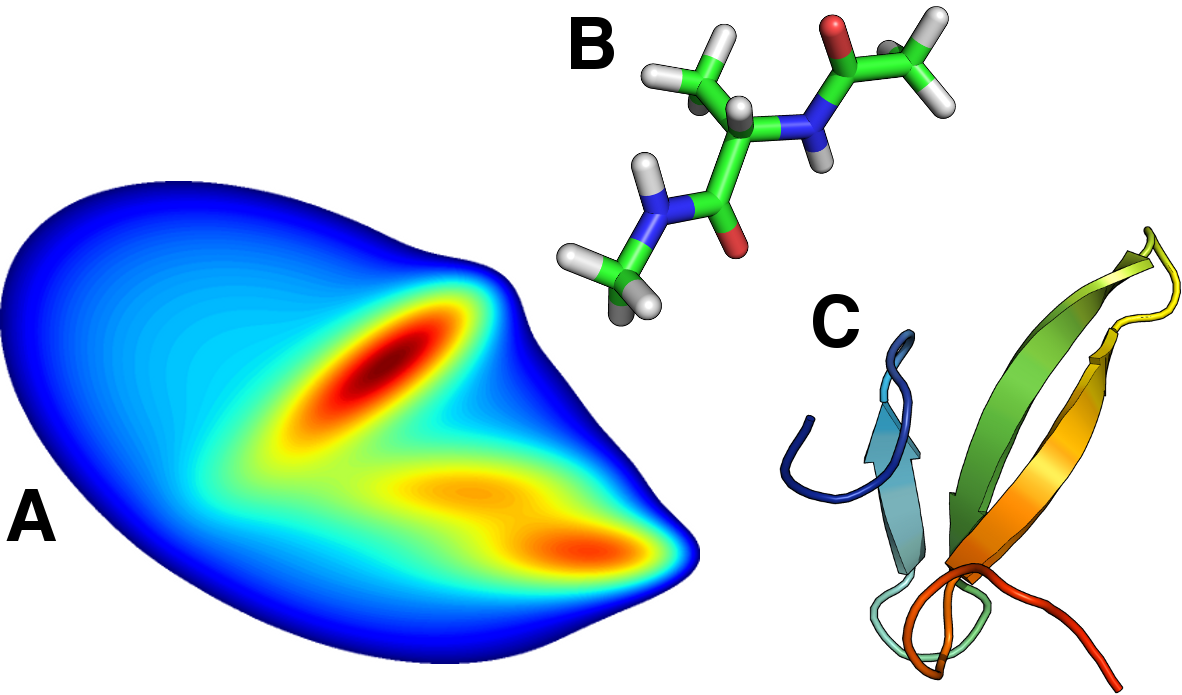
\includegraphics[width=3in]{figs/fig1_rbow.png}
\caption{Three systems studied in this work. (a) Langevin dynamics on the two dimensional M\"{u}ller potential. (b) 50 ns of dynamics of alanine dipeptide. (c) 200 $\mu s$ of dynamics of the Fip35 WW domain\cite{}, courtesy of D.E. Shaw research \cite{}.}
\end{figure}

\section{Results and Discussion}

\bibliography{bibliography}


\end{document}
